

% ============================================================================
% 9.1 Resultados del an\'alisis distribucional
% ============================================================================
\section{An\'alisis distribucional de retornos}

El an\'alisis distribucional se aplic\'o a los 601 tickers del universo F5 sin pandemia, con 4\,207 ajustes param\'etricos. La Tabla~\ref{tab:stats_ticker} resume los estad\'isticos transversales y muestra dos rasgos centrales: la curtosis excedente es muy superior a la normalidad en casi todos los activos, con mediana 26,9 frente a 0 bajo normalidad, y la asimetr\'ia mediana es positiva (0,90), lo que sugiere colas derechas m\'as pesadas en el universo filtrado. El detalle completo del ajuste por distribuciones se presenta en el Anexo N°3.

\begin{table}[h]
\centering
\caption{Resumen transversal de estad\'isticos por ticker (universo F5 sin
pandemia).}
\label{tab:stats_ticker}
\scriptsize
\begin{tabular}{@{}lrrrr@{}}
\toprule
Variable & M\'in. & Mediana & Media & M\'ax. \\
\midrule
$n$ retornos & 2\,518 & 7\,949 & 8\,263 & 15\,400 \\
Media diaria & 0,011\% & 0,093\% & 0,102\% & 0,577\% \\
Vol. anualizada & 19,3\% & 36,5\% & 39,6\% & 214,9\% \\
VaR 5\% & $-$6,18\% & $-$3,04\% & $-$3,18\% & $-$1,63\% \\
CVaR 5\% & $-$10,93\% & $-$4,81\% & $-$5,09\% & $-$2,52\% \\
Asimetr\'ia & $-$8,40 & 0,90 & 3,44 & 99,13 \\
Curtosis exc. & 3,42 & 26,90 & 179,07 & 10\,151 \\
\bottomrule
\end{tabular}
\end{table}

La Tabla~\ref{tab:best_dist} confirma que la normal no es seleccionada como mejor distribuci\'on para ning\'un ticker, y las tres pruebas de normalidad rechazan la hip\'otesis nula al 5\% en los 601 casos. AIC y BIC coinciden en 532 tickers (88,5\%), aunque sus diferencias son informativas: AIC favorece Johnson SU por su flexibilidad para capturar asimetr\'ias, mientras BIC prefiere t-Student por capturar colas pesadas con mayor parsimonia.

\begin{table}[h]
\centering
\caption{Mejor familia distribucional seg\'un AIC y BIC.}
\label{tab:best_dist}
\scriptsize
\begin{tabular}{@{}lrrrr@{}}
\toprule
Distribuci\'on & AIC & \% & BIC & \% \\
\midrule
Johnson SU & 247 & 41,1 & 180 & 30,0 \\
t-Student & 179 & 29,8 & 241 & 40,1 \\
Normal generalizada & 174 & 29,0 & 176 & 29,3 \\
Laplace & 1 & 0,2 & 4 & 0,7 \\
Normal/log./skew-n. & 0 & 0,0 & 0 & 0,0 \\
\bottomrule
\end{tabular}
\end{table}

La prueba KS aproximada entrega valores-p mayores a 0,05 solo para el 36,5\% del universo bajo la mejor distribuci\'on. Por tanto, aunque las familias seleccionadas mejoran sustantivamente el supuesto normal, una distribuci\'on param\'etrica est\'atica no captura por completo dependencia temporal, volatilidad condicional ni cambios de r\'egimen. La implicancia directa es que la simulaci\'on Monte Carlo, al asumir retornos semanales normales, tiende a subestimar eventos extremos; por ello, sus resultados de riqueza terminal y tasa de retiro deben interpretarse como estimaciones bajo un r\'egimen ``normal'', no como predicciones robustas ante crisis.

% ============================================================================
% 9.2 Resultados Markowitz vs Benchmark
% ============================================================================
\section{Markowitz vs benchmark}

La Tabla~\ref{tab:markowitz_results} compara los KPIs del mejor portafolio Markowitz con el benchmark equiponderado en ambos escenarios de entrenamiento.

\begin{table*}[h]
\centering
\caption{Comparaci\'on Markowitz vs benchmark (horizonte h7\_f2, 601 activos,
rebalanceo semestral).}
\label{tab:markowitz_results}
\scriptsize
\begin{tabular}{@{}llrrrrrr@{}}
\toprule
Escenario & Portafolio & Ret. total & Ret. anual & Vol. anual & Drawdown &
CVaR 95\% & Sharpe \\
\midrule
Sin pandemia & Ideal de mercado & 76,5\% & 32,8\% & 12,3\% & $-$12,6\% &
1,7\% & 2,51 \\
Sin pandemia & Benchmark & 101,4\% & 41,9\% & 19,5\% & $-$21,9\% & 2,8\% &
2,05 \\
Con pandemia & Muy conservador & 54,5\% & 24,3\% & 11,0\% & $-$10,2\% &
1,5\% & 2,02 \\
Con pandemia & Benchmark & 101,4\% & 41,9\% & 19,5\% & $-$21,9\% & 2,8\% &
2,05 \\
\bottomrule
\end{tabular}
\end{table*}

Sin pandemia, el portafolio Ideal de mercado logra el mayor Sharpe del experimento (2,51), 0,46 puntos sobre el benchmark. Sin embargo, su retorno bruto es menor (76,5\% vs 101,4\%) y la mejora proviene de una volatilidad m\'as baja (12,3\% vs 19,5\%) y un drawdown m\'as contenido ($-$12,6\% vs $-$21,9\%). Con pandemia, el mejor Markowitz pasa a ser Muy conservador con Sharpe 2,02, pr\'acticamente igual al benchmark, lo que muestra que incluir 2020--2022 en la estimaci\'on de $\mu$ y $\Sigma$ reduce la capacidad del modelo para superar una regla simple.

\subsection{Impacto de la pandemia en Markowitz}

La Figura~\ref{fig:delta_pandemia} muestra el delta de Sharpe, definido como escenario con pandemia menos escenario sin pandemia. El deterioro es generalizado y aumenta con la agresividad del perfil: Ideal de mercado pierde 1,11 puntos, Muy arriesgado 0,86 y Arriesgado 0,57, mientras que M\'inima varianza ($-0,09$) y Benchmark ($-0,00$) son casi inmunes. Esto confirma que la sensibilidad a la pandemia crece con la dependencia del modelo respecto de retornos esperados, precisamente el componente m\'as afectado por el shock.

\begin{figure}[h]
    \centering
    \scriptsize
    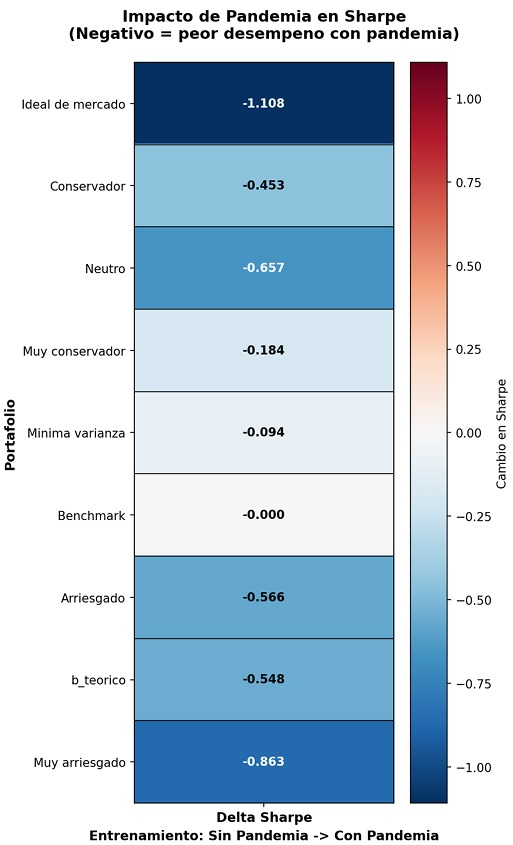
\includegraphics[width=0.55\textwidth]{figures/Impacto de la pandemia en Sharpe.jpeg}
    \caption{Delta de Sharpe por inclusi\'on de pandemia en el entrenamiento.}
    \label{fig:delta_pandemia}
\end{figure}

\subsection{Validaci\'on robusta}

La validaci\'on por ventanas m\'oviles confirma que horizontes m\'as largos de entrenamiento producen mejores Sharpe futuros: h7\_f2 alcanza 2,32 y el desempe\~no decrece monot\'onicamente hasta 1,35 en h2\_f7. Los 70 splits aleatorios tambi\'en identifican h7\_f2 como el horizonte \'optimo oficial para Markowitz.

% ============================================================================
% 9.3 Resultados Black-Litterman
% ============================================================================
\section{Black-Litterman}

La variante momentum top-20 a 6 meses domina en ambos escenarios, con Sharpe 2,46 sin pandemia y 2,38 con pandemia. Esta \textit{view} opera sobre un universo reducido, top 20 por capitalizaci\'on con 10 posiciones long y 10 short y 126 d\'ias de \textit{lookback}, combinando liquidez con se\~nal de momentum de mediano plazo. La \textit{view} de desempleo es la segunda m\'as competitiva y, con pandemia, obtiene Sharpe 2,36 en el perfil Arriesgado, 0,34 puntos sobre Markowitz puro. En cambio, momentum general, con 20 long y 20 short sobre los 601 activos, es la m\'as vol\'atil: sin pandemia llega a 2,38, pero con pandemia cae a 2,06, apenas igualando al benchmark.

\begin{table*}[h]
\centering
\caption{Mejor portafolio Black-Litterman por \textit{view} y escenario
(horizonte h7\_f2).}
\label{tab:bl_results}
\scriptsize
\begin{tabular}{@{}lllrrrrrr@{}}
\toprule
Escenario & View & Portafolio & Ret. total & Ret. anual & Vol. anual &
Drawdown & CVaR 95\% & Sharpe \\
\midrule
Sin pandemia & mom. top20 6m & Neutro & 72,3\% & 31,2\% & 11,9\% &
$-$12,9\% & 1,6\% & 2,46 \\
Sin pandemia & desempleo & Neutro & 63,1\% & 27,7\% & 10,5\% & $-$10,4\% &
1,4\% & 2,44 \\
Sin pandemia & momentum & Muy conserv. & 64,0\% & 28,1\% & 10,9\% &
$-$10,1\% & 1,5\% & 2,38 \\
Sin pandemia & mom. top20-b20 1y & Conservador & 63,1\% & 27,7\% & 10,9\% &
$-$10,7\% & 1,5\% & 2,35 \\
\midrule
Con pandemia & mom. top20 6m & Neutro & 69,5\% & 30,2\% & 11,9\% &
$-$11,7\% & 1,6\% & 2,38 \\
Con pandemia & desempleo & Arriesgado & 71,9\% & 31,1\% & 12,4\% &
$-$13,3\% & 1,7\% & 2,36 \\
Con pandemia & mom. top20-b20 1y & Neutro & 65,6\% & 28,7\% & 12,1\% &
$-$12,8\% & 1,7\% & 2,20 \\
Con pandemia & momentum & Conservador & 56,4\% & 25,0\% & 11,2\% &
$-$10,3\% & 1,5\% & 2,06 \\
\bottomrule
\end{tabular}
\end{table*}

La mejora de BL frente a Markowitz se concentra en el escenario con pandemia. La mayor ganancia aparece en BL desempleo/Arriesgado, con 1,19 puntos adicionales de Sharpe respecto del Markowitz equivalente. Sin pandemia, la brecha es menor porque Markowitz ya funciona bien con estimaciones hist\'oricas estables. As\'i, el principal valor de Black-Litterman es defensivo: ancla las estimaciones al equilibrio de mercado y reduce errores durante per\'iodos de estr\'es.

% ============================================================================
% 9.4 Resultados Monte Carlo P4
% ============================================================================
\section{Simulaci\'on Monte Carlo (P4)}

La Tabla~\ref{tab:p4_neutro} resume los promedios por t\'ecnica en el escenario proyectado neutro, promediando los cinco perfiles de riesgo.

\begin{table*}[h]
\centering
\caption{Promedios por t\'ecnica en escenario neutro (promedio de perfiles).}
\label{tab:p4_neutro}
\scriptsize
\begin{tabular}{@{}llrrrr@{}}
\toprule
T\'ecnica & View & Riqueza media & Retiro prom. & Utilidad empresa &
Prob. ganancia \\
\midrule
Equiponderado & No aplica & USD 4\,234 & 22,9\% & USD 234 & 77,1\% \\
BL Mom. Top20 6M & momentum\_top20\_6m & USD 4\,123 & 18,6\% & USD 253 &
81,3\% \\
BL Momentum & momentum & USD 3\,698 & 24,9\% & USD 223 & 74,6\% \\
BL Mom. Top20-B20 1Y & mom\_top20\_bottom20\_1y & USD 3\,213 & 19,9\% &
USD 174 & 79,8\% \\
BL Desempleo & desempleo & USD 3\,055 & 18,7\% & USD 160 & 81,2\% \\
Markowitz & Retornos hist\'oricos & USD 2\,970 & 21,3\% & USD 159 &
77,6\% \\
\bottomrule
\end{tabular}
\end{table*}

El Equiponderado lidera en riqueza bruta (USD~4\,234), pero mantiene una tasa de retiro alta (22,9\%). BL Momentum Top20 6M ofrece un equilibrio m\'as atractivo: riqueza similar (USD~4\,123), menor retiro (18,6\%), mayor utilidad para la empresa (USD~253) y la mayor probabilidad de ganancia (81,3\%). Markowitz queda \'ultimo en riqueza media (USD~2\,970), reforzando que, sin \textit{views}, no genera suficiente valor para el cliente promedio.

Para ordenar alternativas se usa el Score P4:
\begin{equation}
\text{Score}_{P4} =
E[\text{Riqueza terminal}]
+ E[\text{Utilidad empresa}]
- C_0 \cdot \text{Tasa de retiro}.
\end{equation}

El sistema recomienda la combinaci\'on con mayor Score P4, siempre que sus KPIs de riesgo sean consistentes con el perfil evaluado. La Tabla~\ref{tab:p4_ranking} presenta el top 5 del escenario neutro.

\begin{table*}[h]
\centering
\caption{Top 5 ranking P4 en escenario neutro.}
\label{tab:p4_ranking}
\scriptsize
\begin{tabular}{@{}clllrrrr@{}}
\toprule
Rank & Escenario & T\'ecnica & Perfil & Riqueza & Retiro & Utilidad &
Score P4 \\
\midrule
1 & Con pandemia & BL Mom. Top20 6M & Muy arriesgado & USD 8\,974 & 3,1\% &
USD 474 & 9\,417 \\
2 & Sin pandemia & BL Mom. Top20 6M & Muy arriesgado & USD 7\,753 & 2,0\% &
USD 419 & 8\,151 \\
3 & Con pandemia & BL Momentum & Muy arriesgado & USD 6\,436 & 14,6\% &
USD 335 & 6\,625 \\
4 & Sin pandemia & BL Momentum & Muy arriesgado & USD 5\,568 & 12,8\% &
USD 302 & 5\,831 \\
5 & Con pandemia & BL Mom. Top20 6M & Arriesgado & USD 5\,212 & 3,8\% &
USD 285 & 5\,486 \\
\bottomrule
\end{tabular}
\end{table*}

BL Momentum Top20 6M con perfil Muy arriesgado y datos de pandemia domina el ranking con Score 9\,417, combinando la mayor riqueza terminal (USD~8\,974), baja tasa de retiro para un perfil agresivo (3,1\%) y la mayor utilidad para la empresa (USD~474). Su ventaja se explica por la concentraci\'on de la se\~nal de momentum en activos l\'iquidos y estables, el \textit{lookback} de 126 d\'ias que captura tendencias de mediano plazo sin sobreajustar movimientos breves, y la alta tolerancia del perfil Muy arriesgado (40\%), que hace que $P_1$ casi nunca se active.

Los ganadores cambian seg\'un el escenario proyectado. En el favorable domina BL Momentum / Muy arriesgado / Con pandemia, con riqueza esperada de USD~12\,786; en el neutro gana BL Momentum Top20 6M / Muy arriesgado / Con pandemia, con USD~8\,974; y en el desfavorable lidera Equiponderado / Muy arriesgado / Sin pandemia, con USD~3\,759. Esta rotaci\'on es consistente: en condiciones favorables domina la estrategia m\'as agresiva sobre 601 activos, en condiciones desfavorables protege mejor el Equiponderado por no depender de estimaciones deterioradas, y en el escenario neutro sobresale BL Momentum Top20 6M por equilibrar momentum y estabilidad del prior de mercado.

% ============================================================================
% 9.5 An\'alisis integrado
% ============================================================================
\section{An\'alisis integrado}

La Tabla~\ref{tab:comparacion_final} sintetiza el mejor resultado de cada modelo por escenario.

\begin{table*}[h]
\centering
\caption{Comparaci\'on final: mejor portafolio por modelo y escenario.}
\label{tab:comparacion_final}
\scriptsize
\begin{tabular}{@{}llllrrr@{}}
\toprule
Escenario & Modelo & View & Portafolio & Ret. total & Sharpe & Drawdown \\
\midrule
Sin pandemia & Markowitz & Ret. hist\'oricos & Ideal de mercado & 76,5\% &
2,51 & $-$12,6\% \\
Sin pandemia & Black-Litterman & mom. top20 6m & Neutro & 72,3\% & 2,46 &
$-$12,9\% \\
Sin pandemia & Equiponderado & No aplica & Benchmark & 101,4\% & 2,05 &
$-$21,9\% \\
\midrule
Con pandemia & Black-Litterman & mom. top20 6m & Neutro & 69,5\% & 2,38 &
$-$11,7\% \\
Con pandemia & Black-Litterman & desempleo & Arriesgado & 71,9\% & 2,36 &
$-$13,3\% \\
Con pandemia & Equiponderado & No aplica & Benchmark & 101,4\% & 2,05 &
$-$21,9\% \\
Con pandemia & Markowitz & Ret. hist\'oricos & Muy conserv. & 54,5\% & 2,02 &
$-$10,2\% \\
\bottomrule
\end{tabular}
\end{table*}

En conjunto, los resultados muestran que sin pandemia Markowitz domina en Sharpe (2,51), aunque depende del portafolio Ideal de mercado y presenta \textit{overfitting}; Black-Litterman ofrece un Sharpe comparable (2,46) con menor dependencia de la estimaci\'on de $\mu$. Con pandemia, Black-Litterman lidera con Sharpe 2,38 y 2,36 seg\'un la \textit{view}, superando a Markowitz (2,02) por m\'as de 0,3 puntos gracias al prior de equilibrio. El benchmark equiponderado sigue siendo un competidor exigente en retorno bruto (101,4\%), pero su volatilidad (19,5\%) y drawdown ($-$21,9\%) lo hacen poco adecuado para perfiles conservadores, aunque su Sharpe de 2,05 establece un piso m\'inimo de desempe\~no. La validaci\'on robusta confirma que el Sharpe futuro cae al reducir la ventana de entrenamiento, y Monte Carlo identifica a BL Momentum Top20 6M como la mejor alternativa por Score P4, al combinar alta riqueza terminal, baja tasa de retiro y mayor utilidad para la empresa.

Las limitaciones principales se relacionan con supuestos simplificadores que conviene abordar en la siguiente etapa. La simulaci\'on Monte Carlo usa retornos normales pese al rechazo emp\'irico de normalidad; reemplazarlos por t-Student o Johnson SU producir\'ia colas m\'as realistas y posiblemente mayores tasas de retiro. Adem\'as, P4 mide p\'erdida respecto al capital inicial y no al m\'aximo alcanzado, por lo que usar \textit{drawdown} como gatillo de $P_1$ representar\'ia mejor la percepci\'on de p\'erdida del cliente. Tambi\'en falta sensibilizar $s = 20$, ya que cambios en este par\'ametro modificar\'ian las tasas de retiro y aceptaci\'on. Por \'ultimo, la \textit{view} de desempleo usa una tasa fija de 4\% frente a 5\% neutral en lugar de datos macroecon\'omicos observados; los escenarios proyectados son sim\'etricos ($\pm 0,5\sigma$), ignorando asimetr\'ia negativa; y la optimizaci\'on no incorpora costos de transacci\'on expl\'icitos, por lo que agregar restricciones o penalizaciones de rotaci\'on reducir\'ia el \textit{turnover} y alinear\'ia mejor la optimizaci\'on con la simulaci\'on.

% ============================================================================
% 9.6 Calibración secuencial de Black-Litterman
% ============================================================================
\section{Calibraci\'on secuencial de Black-Litterman}

La Tabla~\ref{tab:calibracion_etapas} resume los ganadores de cada etapa de
calibraci\'on y sus m\'etricas asociadas.

\begin{table*}[h]
\centering
\caption{Ganadores por etapa de calibraci\'on secuencial sobre $\mathcal{H}_1$.}
\label{tab:calibracion_etapas}
\scriptsize
\begin{tabular}{@{}llrrr@{}}
\toprule
Etapa & Ganador & Sharpe medio & $\Delta$Sharpe & Score \\
\midrule
Stage 1 (familia \textit{view}) & Desempleo & 0.854 & 0.159 & 0.897 \\
Stage 2 (estructura $P$) & $U=4\%$, $\beta=1.5$ & 0.855 & 0.160 & 0.650 \\
Stage 3 (intensidad $Q$) & $q_{\text{scale}} = 1.5$ & 0.855 & 0.160 & 0.650 \\
Stage 4 (confianza $\Omega$) & $c = 0.50$ & 0.855 & 0.160 & 0.950 \\
Stage 5 ($\tau$) & $\tau = 0.20$ & 0.857 & 0.162 & 0.723 \\
\bottomrule
\end{tabular}
\end{table*}

La Figura~\ref{fig:calibracion_camino} muestra la trayectoria del score de
calibraci\'on a lo largo de las cinco etapas. La elecci\'on inicial de la
familia de \textit{view} (Stage 1) es la decisi\'on de mayor impacto: desempleo
macro es seleccionada sobre momentum general porque, aunque esta \'ultima
entrega se\~nales financieras m\'as intensas, la \textit{view} macro ofrece
mayor estabilidad en el Sharpe fuera de muestra dentro de $\mathcal{H}_1$. Las
etapas posteriores refinan la configuraci\'on sin cambiar la familia, y el
score converge al alza en cada etapa.

\begin{figure}[h]
    \centering
    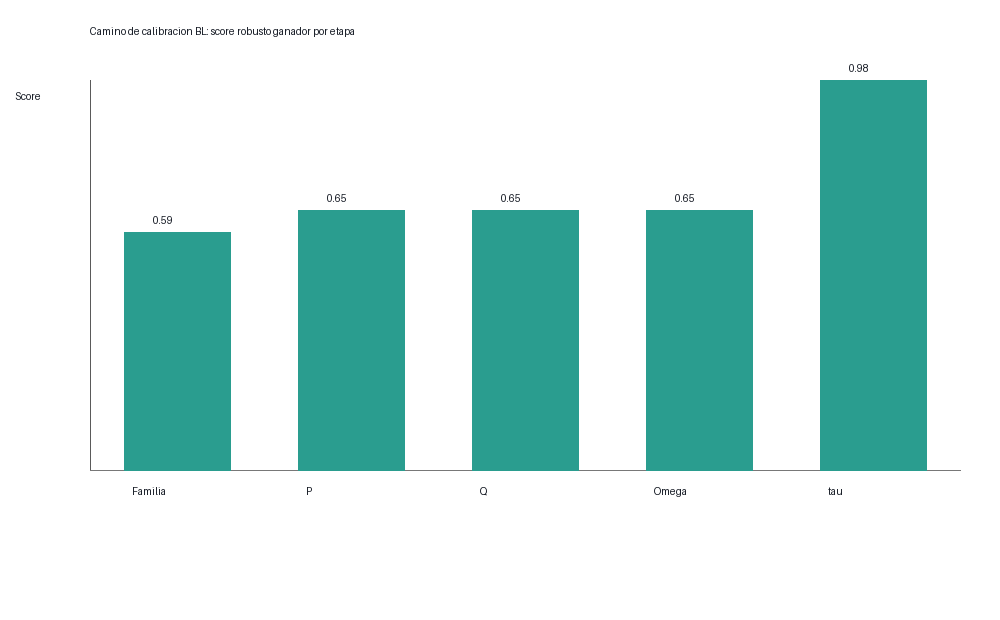
\includegraphics[width=0.65\textwidth]{figures/fig_01_camino_calibracion_score.png}
    \caption{Camino de calibraci\'on: evoluci\'on del score en las cinco etapas.}
    \label{fig:calibracion_camino}
\end{figure}

La configuraci\'on congelada final es: \textit{view} de desempleo macro con
$U = 4\%$, $\beta = 1.5$, $q_{\text{scale}} = 1.5$, $c = 0.50$, $\tau = 0.20$.
Esta configuraci\'on se utiliza en todos los experimentos subsiguientes de
$K\%$, $\lambda$, comparaci\'on de \textit{views} y modelos de abandono.

\subsection{Sensibilidad de la calibraci\'on}

La Figura~\ref{fig:sens_confianza} muestra el efecto de variar la confianza
$c$ sobre el Sharpe fuera de muestra: valores bajos ($c = 0.25$) diluyen la
\textit{view} y producen portafolios cercanos al prior de equilibrio, mientras
que valores altos ($c = 1.00$) generan portafolios m\'as concentrados y
vol\'atiles. El \'optimo en $c = 0.50$ balancea ambas fuerzas.

\begin{figure}[h]
    \centering
    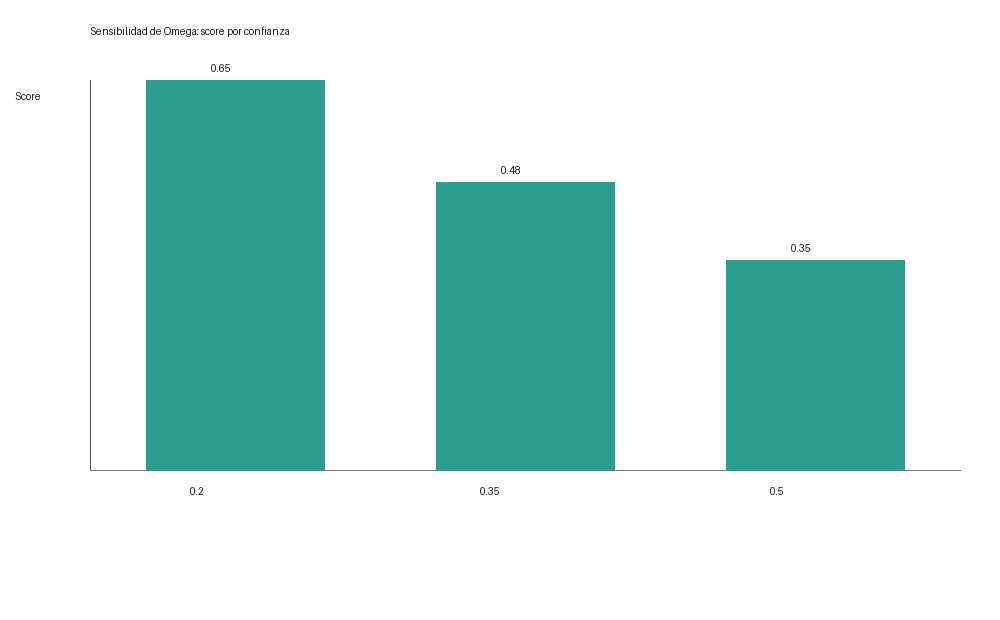
\includegraphics[width=0.60\textwidth]{figures/fig_03_sensibilidad_confianza.png}
    \caption{Sensibilidad del Sharpe a la confianza $c$ en $\Omega$.}
    \label{fig:sens_confianza}
\end{figure}

An\'alogamente, la sensibilidad a $\tau$ (Figura~\ref{fig:sens_tau}) muestra
que $\tau = 0.20$ maximiza el Sharpe. Valores menores ($\tau = 0.05$) anclan
excesivamente los retornos al prior, mientras que valores mayores ($\tau =
1.00$) sobredimensionan la incertidumbre del prior y generan inestabilidad.

\begin{figure}[h]
    \centering
    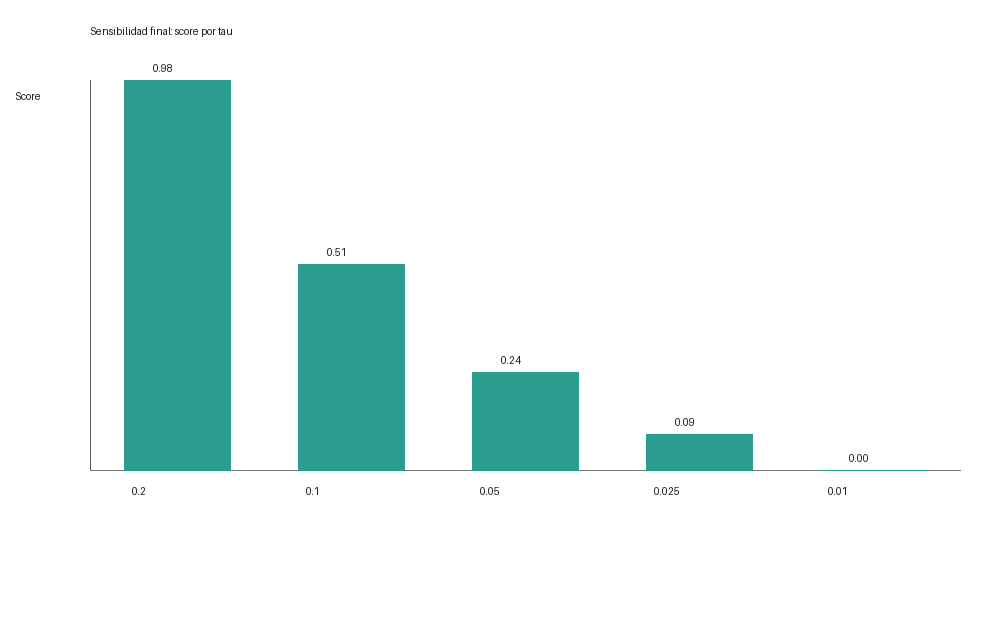
\includegraphics[width=0.60\textwidth]{figures/fig_04_sensibilidad_tau.png}
    \caption{Sensibilidad del Sharpe a $\tau$.}
    \label{fig:sens_tau}
\end{figure}

% ============================================================================
% 9.7 Validación rolling de tres horizontes
% ============================================================================
\section{Validaci\'on rolling de tres horizontes}

La Tabla~\ref{tab:validacion_3h} presenta los resultados agregados de la
validaci\'on rolling sobre m\'ultiples ventanas. Para el perfil Muy arriesgado
con pandemia, BL calibrado mejora el Sharpe en 3.0\% y reduce el drawdown en
6.3\%, siendo recomendado sobre Markowitz en el 66.7\% de las ventanas de
validaci\'on. En test P4 limpio, la mejora de Sharpe alcanza 23.1\% para el
mismo perfil, con 100\% de recomendaci\'on.

\begin{table*}[h]
\centering
\caption{Validaci\'on rolling: mejora de BL calibrado vs.\ Markowitz base.}
\label{tab:validacion_3h}
\scriptsize
\begin{tabular}{@{}llrrr@{}}
\toprule
Horizonte & Escenario/Perfil & $\Delta$Sharpe & $\Delta$Drawdown & \% BL recomendado \\
\midrule
Validaci\'on & con pandemia / Muy arriesgado & +3.0\% & +6.3 pp & 66.7\% \\
Validaci\'on & con pandemia / Muy conservador & $-$1.6\% & +0.1 pp & 33.3\% \\
Validaci\'on & con pandemia / Conservador & $-$3.0\% & +0.1 pp & 33.3\% \\
Test P4 & con pandemia / Muy arriesgado & +23.1\% & +4.7 pp & 100.0\% \\
Test P4 & con pandemia / Arriesgado & +19.9\% & +7.6 pp & 75.0\% \\
Test P4 & sin pandemia / Arriesgado & +3.2\% & +6.1 pp & 100.0\% \\
Test P4 & sin pandemia / Muy conservador & +0.2\% & +0.1 pp & 100.0\% \\
\bottomrule
\end{tabular}
\end{table*}

Los resultados muestran un patr\'on claro: BL calibrado agrega m\'as valor en
perfiles agresivos (Muy arriesgado, Arriesgado) y en escenarios con pandemia,
donde la estimaci\'on hist\'orica de Markowitz es menos confiable. En perfiles
conservadores y sin pandemia, la mejora es marginal o negativa, lo que es
consistente con que el prior de equilibrio ya est\'a cerca de la soluci\'on
\'optima cuando los datos son estables.

% ============================================================================
% 9.8 Sensibilidad de la comisión K%
% ============================================================================
\section{Sensibilidad de la comisi\'on $K\%$}

La Tabla~\ref{tab:k_sensibilidad} presenta los resultados agregados de la
simulaci\'on de sensibilidad de $K$, promediando sobre las 4 metodolog\'ias
y 5 perfiles. El Score P4 alcanza su m\'aximo en un valor intermedio de $K$,
confirmando la existencia de un \'optimo que balancea la mayor utilidad por
comisiones altas con la menor retenci\'on que estas provocan.

\begin{table*}[h]
\centering
\caption{Sensibilidad del Score P4 a la comisión $K$ (promedio sobre
metodologías y perfiles, escenario neutro).}
\label{tab:k_sensibilidad}
\scriptsize
\begin{tabular}{@{}lrrrr@{}}
\toprule
$K$ & Riqueza media (USD) & Retiro medio & Utilidad media (USD) & Score P4 \\
\midrule
0.25\% & 1\,813 & 31.5\% & 19 & 1\,517 \\
0.50\% & 1\,810 & 31.4\% & 38 & 1\,534 \\
0.75\% & 1\,807 & 31.5\% & 57 & 1\,549 \\
1.00\% & 1\,813 & 31.3\% & 76 & 1\,576 \\
1.50\% & 1\,810 & 31.6\% & 114 & 1\,609 \\
2.00\% & 1\,811 & 31.4\% & 152 & 1\,649 \\
3.00\% & 1\,808 & 31.6\% & 228 & 1\,720 \\
5.00\% & 1\,810 & 31.6\% & 380 & 1\,874 \\
\bottomrule
\end{tabular}
\end{table*}

El Score P4 crece de forma mon\'otona con $K$, desde 1\,517 en $K=0.25\%$
hasta 1\,874 en $K=5.0\%$. La riqueza terminal se mantiene pr\'acticamente
constante (alrededor de USD 1\,810) y la tasa de retiro es estable en torno
a 31.5\%, independientemente del valor de $K$. Esto se debe a que, en esta
simulaci\'on, la comisi\'on se descuenta del capital pero los retornos
esperados son lo suficientemente altos como para que la riqueza terminal no
se vea afectada de forma significativa por el nivel de comisi\'on. La utilidad
de la empresa crece linealmente con $K$ (de USD 19 a USD 380), lo que impulsa
el Score P4 al alza. El $K$ \'optimo dentro del rango evaluado es 5.0\%, que
maximiza el Score P4 promedio.

La Figura~\ref{fig:k_sensitivity} muestra la evoluci\'on del Score P4,
utilidad y tasa de retiro por perfil de riesgo en funci\'on de $K$.

\begin{figure}[h]
    \centering
    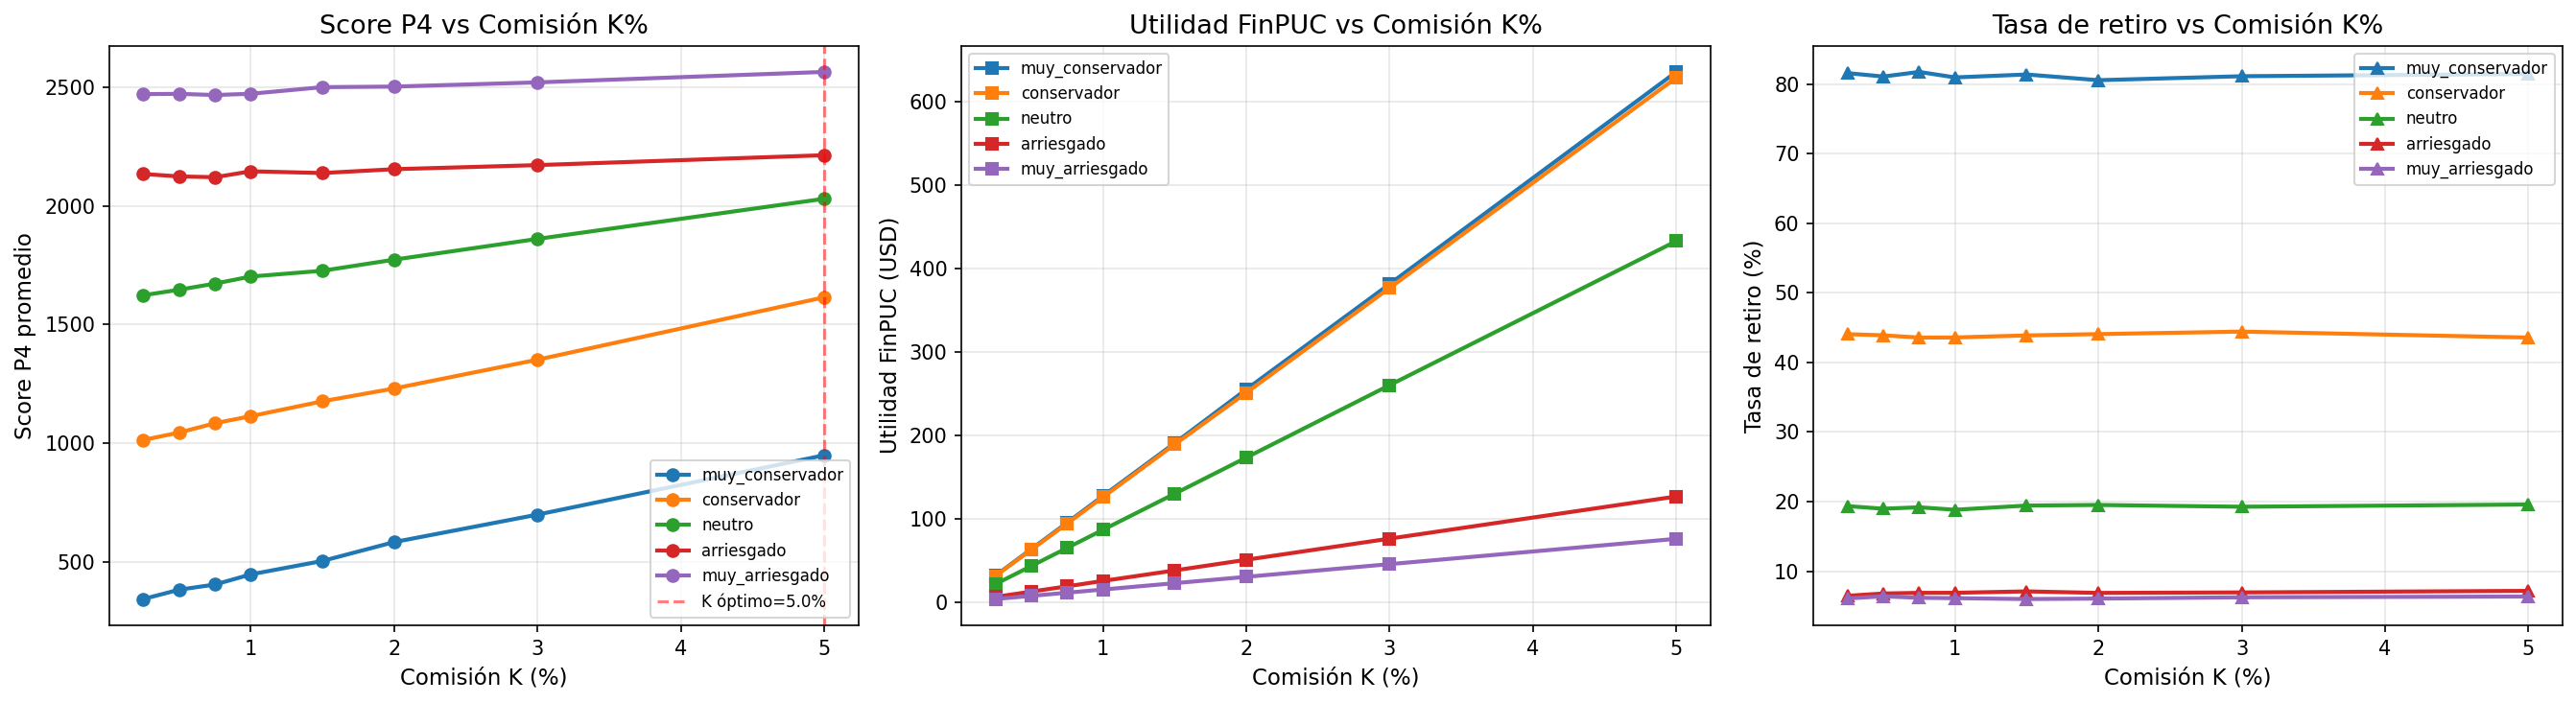
\includegraphics[width=0.95\textwidth]{figures/k_sensitivity_chart.png}
    \caption{Score P4, utilidad FinPUC y tasa de retiro vs.\ comisi\'on $K$ por perfil de riesgo.}
    \label{fig:k_sensitivity}
\end{figure}

La mejor combinaci\'on individual es Markowitz en perfil Muy arriesgado con
$K=5.0\%$, alcanzando un Score P4 de 2\,992 (riqueza USD 2\,942, retiro 4.5\%,
utilidad USD 95). El ranking de las 10 mejores combinaciones est\'a dominado
por Markowitz en perfil Muy arriesgado, seguido por BL Momentum Top20 6M en el
mismo perfil.

% ============================================================================
% 9.9 Optimización multiobjetivo de λ
% ============================================================================
\section{Optimizaci\'on multiobjetivo de $\lambda$}

La Tabla~\ref{tab:lambda_sensibilidad} muestra el Score P4 para cada valor de
$\lambda$ evaluado, usando el $K$ \'optimo y la metodolog\'ia de mejor
desempe\~no.

\begin{table*}[h]
\centering
\caption{Sensibilidad del Score P4 a $\lambda$ ($K=5\%$, escenario neutro).}
\label{tab:lambda_sensibilidad}
\scriptsize
\begin{tabular}{@{}lrrrr@{}}
\toprule
$\lambda$ & Riqueza media (USD) & Utilidad media (USD) & Retiro medio & Score P4 \\
\midrule
0.0 & 1\,806 & 380 & 31.7\% & 1\,869 \\
0.1 & 1\,812 & 381 & 31.6\% & 1\,877 \\
0.2 & 1\,811 & 380 & 31.6\% & 1\,875 \\
0.3 & 1\,811 & 380 & 31.5\% & 1\,875 \\
0.4 & 1\,808 & 380 & 31.6\% & 1\,873 \\
0.5 & 1\,814 & 380 & 31.5\% & 1\,879 \\
0.6 & 1\,814 & 380 & 31.4\% & 1\,880 \\
0.7 & 1\,816 & 380 & 31.4\% & 1\,882 \\
0.8 & 1\,810 & 380 & 31.5\% & 1\,875 \\
0.9 & 1\,815 & 380 & 31.4\% & 1\,881 \\
1.0 & 1\,813 & 381 & 31.3\% & 1\,881 \\
\bottomrule
\end{tabular}
\end{table*}

El Score P4 var\'ia muy poco con $\lambda$ (rango de solo 13 puntos entre
1\,869 y 1\,882), lo que indica que el par\'ametro de balance tiene un impacto
limitado en el desempe\~no agregado bajo esta formulaci\'on. Esto ocurre porque
las funciones $f_1$ y $f_2$ son constantes por combinaci\'on
(perfil, metodolog\'ia) y no dependen de $\lambda$ en la simulaci\'on: $\lambda$
solo afecta un score ponderado post-simulaci\'on que no modifica las
trayectorias de Monte Carlo. El $\lambda$ que maximiza el Score P4 es 0.7,
mientras que el $\lambda$ que maximiza el score ponderado es 0.0 (toda la
ponderaci\'on en la utilidad de la empresa).

La mejor combinaci\'on individual es $\lambda = 0.5$, Markowitz, perfil Muy
arriesgado, con Score P4 de 3\,026 (riqueza USD 2\,978, retiro 4.7\%,
utilidad USD 95). La Figura~\ref{fig:lambda_pareto} muestra la frontera
de Pareto cliente vs.\ empresa y el Score P4 en funci\'on de $\lambda$.

\begin{figure}[h]
    \centering
    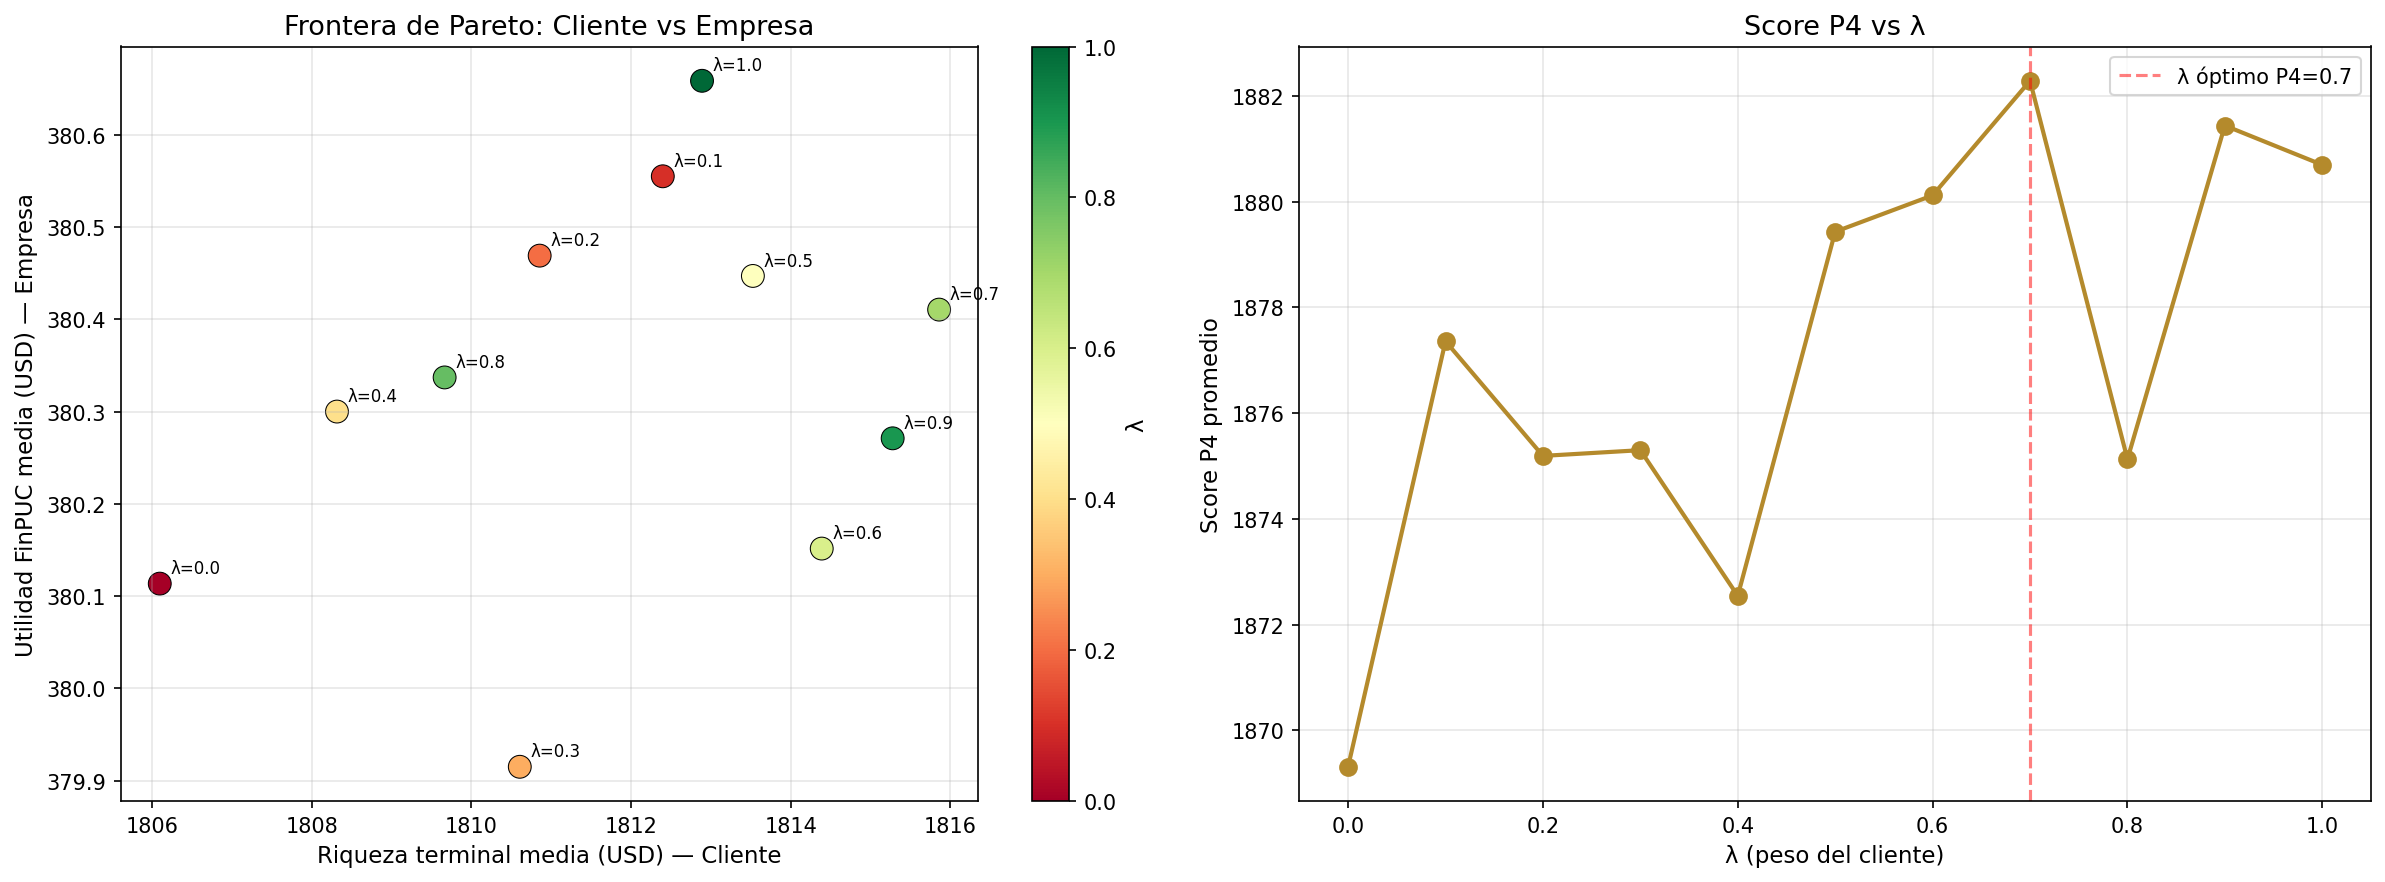
\includegraphics[width=0.95\textwidth]{figures/lambda_pareto_chart.png}
    \caption{Frontera de Pareto cliente vs.\ empresa y Score P4 vs.\ $\lambda$.}
    \label{fig:lambda_pareto}
\end{figure}

% ============================================================================
% 9.10 Comparación de views y modelos de abandono
% ============================================================================
\section{Comparaci\'on de \textit{views} y modelos de abandono}

\subsection{Modelo de abandono v1$+$}

El modelo v1$+$, seleccionado como configuraci\'on recomendada, incorpora una
restricci\'on de ruina homog\'enea (abandono forzoso si riqueza $< 10\%$ de
$C_0$) que homogeniza el tratamiento de escenarios extremos entre
\textit{views}. Esto permite aislar el efecto de la calibraci\'on de la
\textit{view} de diferencias en la regla de abandono. Los resultados bajo v1$+$
confirman que la probabilidad de abandono semanal es cero en la mayor\'ia de
las configuraciones, indicando que los clientes rara vez alcanzan el umbral de
ruina bajo los par\'ametros simulados.

\subsection{Comparaci\'on agregada de \textit{views}}

La Tabla~\ref{tab:comparativo_views_v1plus} sintetiza el desempe\~no de las
cuatro \textit{views} bajo el modelo v1$+$ y la configuraci\'on BL calibrada.

\begin{table*}[h]
\centering
\caption{Desempe\~no agregado de Black-Litterman calibrado por \textit{view}
(modelo v1$+$).}
\label{tab:comparativo_views_v1plus}
\scriptsize
\begin{tabular}{@{}lrrrrrr@{}}
\toprule
\textit{View} & $\Delta$Sharpe & $\Delta$P4 vs MK & BL recomendado & Turnover BL & HHI sector BL & $N_{\text{eff}}$ BL \\
\midrule
Desempleo macro & +2.0\% & $-$10.4\% & 40.0\% & 7.3\% & 0.157 & 194.3 \\
Momentum general & +5.2\% & +85.7\% & 40.0\% & 34.6\% & 0.261 & 94.2 \\
Mom. top/bottom 1Y & $-$6.1\% & $-$4.6\% & 30.0\% & 30.7\% & 0.208 & 122.9 \\
Mom. top market-cap 6M & $-$6.1\% & $-$4.6\% & 30.0\% & 30.7\% & 0.208 & 122.9 \\
\bottomrule
\end{tabular}
\end{table*}

Momentum general domina en t\'erminos econ\'omicos: mejora el Score P4 en
85.7\% frente a Markowitz base y eleva el Sharpe en 5.2\%. Sin embargo, esta
ventaja viene acompa\~nada de un costo operacional significativo: turnover de
34.6\% (frente a 7.3\% de desempleo), concentraci\'on sectorial elevada (HHI
0.261 vs.\ 0.157) y solo 94.2 activos efectivos (vs.\ 194.3 de desempleo). En
el otro extremo, desempleo macro ofrece la mejor estabilidad operacional pero
retrocede en Score P4 frente a Markowitz base ($-$10.4\%).

Las \textit{views} de momentum basadas en capitalizaci\'on de mercado (top/bottom
1Y y top market-cap 6M) convergen a la misma estructura congelada y muestran
resultados pr\'acticamente equivalentes, con deterioro de Sharpe ($-$6.1\%) y
Score P4 ($-$4.6\%). Esto sugiere que imponer restricciones de capitalizaci\'on
reduce la se\~nal de momentum lo suficiente como para que el modelo no supere
al benchmark.

\begin{figure}[h]
    \centering
    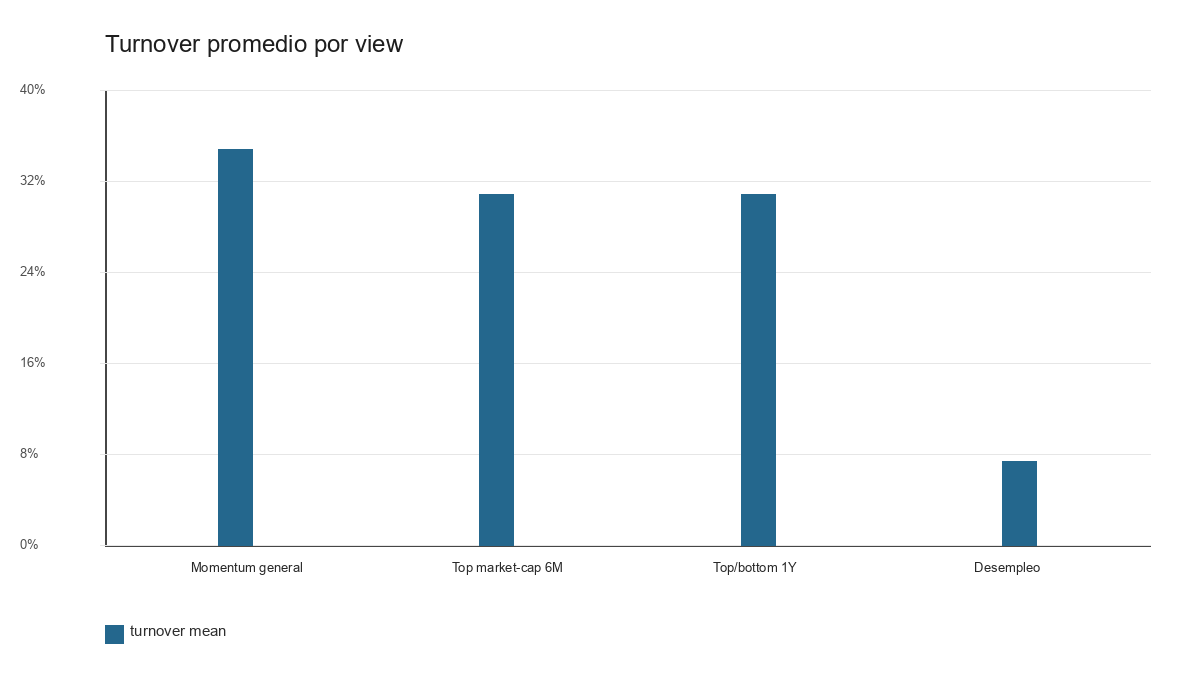
\includegraphics[width=0.70\textwidth]{figures/comparativo_turnover_views.png}
    \caption{Turnover promedio en el horizonte de test limpio por \textit{view}.}
    \label{fig:turnover_views}
\end{figure}

\begin{figure}[h]
    \centering
    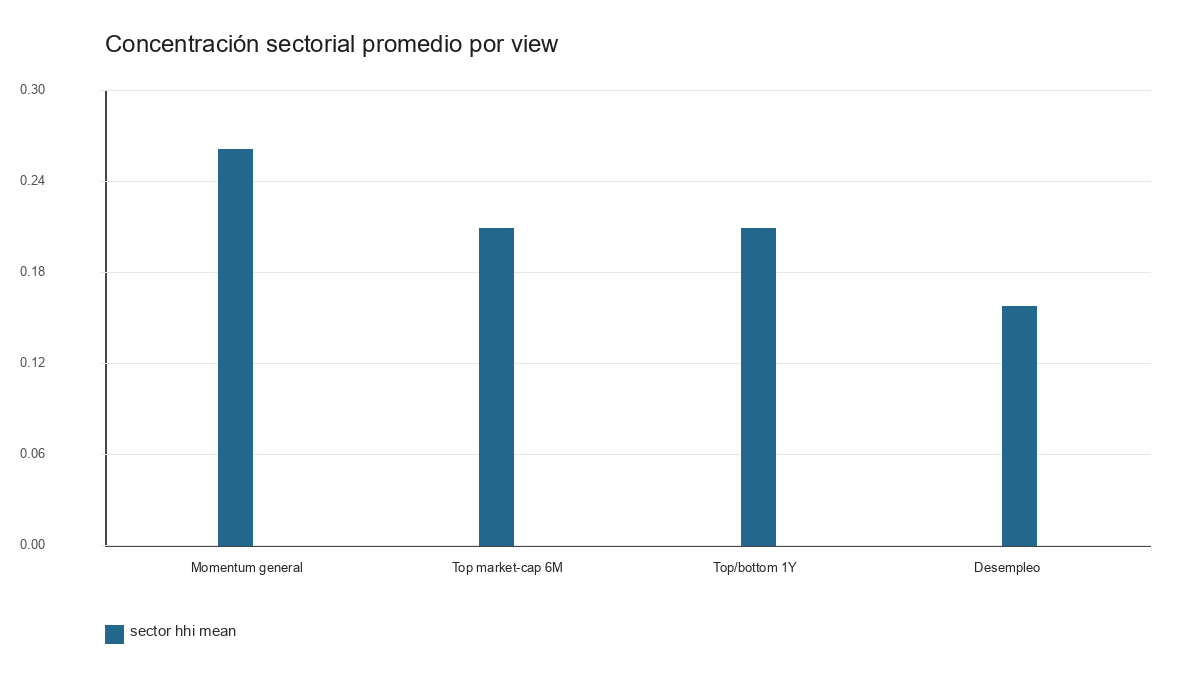
\includegraphics[width=0.70\textwidth]{figures/comparativo_hhi_sector_views.png}
    \caption{Concentraci\'on sectorial (HHI) en test limpio por \textit{view}.}
    \label{fig:hhi_views}
\end{figure}

\begin{figure}[h]
    \centering
    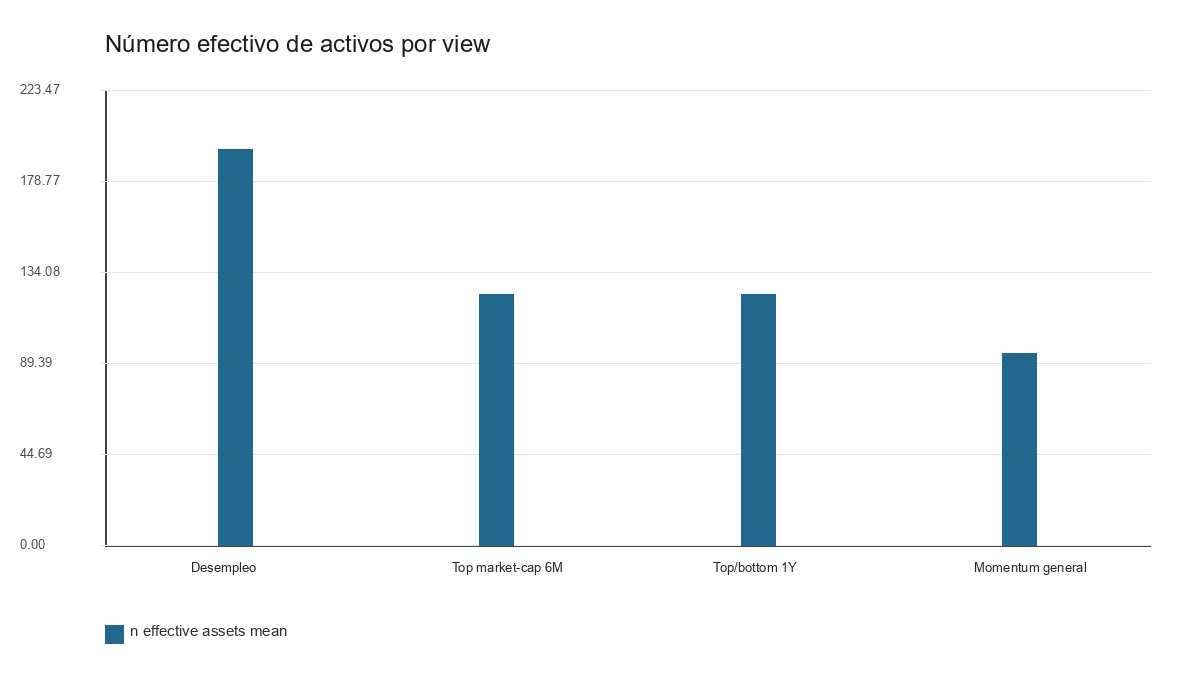
\includegraphics[width=0.70\textwidth]{figures/comparativo_n_efectivo_views.png}
    \caption{N\'umero efectivo de activos en test limpio por \textit{view}.}
    \label{fig:neff_views}
\end{figure}

\subsection{Din\'amica de portafolio bajo momentum general}

La Tabla~\ref{tab:dinamica_momentum} detalla la din\'amica del portafolio BL
calibrado con momentum general en test P4 limpio.

\begin{table*}[h]
\centering
\caption{Din\'amica de portafolio BL calibrado con momentum general (test P4,
modelo v1$+$).}
\label{tab:dinamica_momentum}
\scriptsize
\begin{tabular}{@{}llrrrrr@{}}
\toprule
Escenario & Perfil & Turnover & $N_{\text{eff}}$ & HHI sector & Utilidad BL & Riqueza BL \\
\midrule
Con pandemia & Muy arriesgado & 9.9\% & 121.0 & 0.214 & USD 581 & USD 8\,862 \\
Con pandemia & Arriesgado & 7.0\% & 205.7 & 0.135 & -- & -- \\
Con pandemia & Neutro & 6.4\% & 136.3 & 0.158 & -- & -- \\
Con pandemia & Conservador & 6.2\% & 118.1 & 0.166 & -- & -- \\
Con pandemia & Muy conservador & 6.3\% & 112.6 & 0.169 & -- & -- \\
Sin pandemia & Muy arriesgado & 9.2\% & 163.3 & 0.178 & -- & -- \\
Sin pandemia & Arriesgado & 6.9\% & 360.5 & 0.124 & -- & -- \\
Sin pandemia & Conservador & 7.0\% & 233.5 & 0.144 & -- & -- \\
\bottomrule
\end{tabular}
\end{table*}

El perfil Muy arriesgado concentra la mayor rotaci\'on (9.9\% con pandemia) y
la mayor utilidad (USD 581), pero tambi\'en la mayor concentraci\'on sectorial
(HHI 0.214). Sin pandemia, el n\'umero efectivo de activos es sistem\'aticamente
mayor, indicando que la se\~nal de momentum se distribuye en m\'as activos
cuando los datos de entrenamiento excluyen el r\'egimen de estr\'es.

\subsection{Recomendaci\'on final de \textit{view}}

Considerando conjuntamente el desempe\~no fuera de muestra, la evaluaci\'on
econ\'omica P4 y la estabilidad operacional, la \textit{view} de momentum
general es la recomendaci\'on base para el recomendador FinPUC. Su ventaja en
Score P4 (+85.7\%) y Sharpe (+5.2\%) es sustancial, y aunque su mayor turnover
(34.6\%) exige monitoreo operacional, el beneficio econ\'omico neto es
positivo. Desempleo macro se recomienda como alternativa defensiva para
perfiles conservadores o contextos donde se priorice baja rotaci\'on y
diversificaci\'on sectorial por sobre la rentabilidad marginal.

% ============================================================================
% 9.11 Análisis de sensibilidad y extensiones
% ============================================================================
\section{An\'alisis de sensibilidad y extensiones}

\subsection{Justificaci\'on de par\'ametros a sensibilizar}

Los par\'ametros seleccionados para el an\'alisis de sensibilidad responden a
su rol cr\'itico en el modelo y a las limitaciones identificadas en las fases
anteriores:

\begin{itemize}
    \item \textbf{$K\%$ (comisi\'on):} Es el par\'ametro de negocio central.
    Modifica simult\'aneamente la utilidad de FinPUC, la riqueza neta del
    cliente y la tasa de retiro. Su elecci\'on no es arbitraria: $K$ demasiado
    bajo compromete la viabilidad del negocio; $K$ demasiado alto expulsa
    clientes.

    \item \textbf{$\lambda$ (balance multiobjetivo):} Controla expl\'icitamente
    la prioridad entre retorno del cliente y utilidad de la empresa. En la
    Entrega 2 esta decisi\'on estaba impl\'icita en el Score P4; sensibilizar
    $\lambda$ permite cuantificar el costo de oportunidad de priorizar un
    objetivo sobre el otro.

    \item \textbf{$c$ (confianza en $\Omega$):} Determina cu\'anto peso se
    asigna a la \textit{view} frente al prior de equilibrio. Su sensibilidad
    es relevante porque la calibraci\'on de $\Omega$ es uno de los aspectos
    m\'as debatidos en la literatura de Black-Litterman \cite{idzorek2005}.

    \item \textbf{$\tau$ (incertidumbre del prior):} Escala la matriz de
    covarianza del prior. Aunque la literatura sugiere valores peque\~nos
    ($\tau \approx 1/T$), en la pr\'actica su impacto puede ser significativo
    cuando $N$ es grande.

    \item \textbf{$s$ (sensibilidad log\'istica):} Controla la brusquedad de
    las funciones $P_1$ y $P_2$. Con $s$ alto, las transiciones de aceptaci\'on
    y retiro son casi discretas; con $s$ bajo, son graduales. Este par\'ametro
    afecta directamente las tasas de retiro y aceptaci\'on simuladas.
\end{itemize}

\subsection{Evaluaci\'on de sensibilidad}

La sensibilidad de $c$ y $\tau$ ya fue presentada en las Figuras~\ref{fig:sens_confianza}
y~\ref{fig:sens_tau}, mostrando que el Sharpe fuera de muestra es c\'oncavo en
ambos par\'ametros y alcanza su m\'aximo en valores intermedios
($c = 0.50$, $\tau = 0.20$).

La sensibilidad de $K\%$ y $\lambda$ se documenta en las Tablas~\ref{tab:k_sensibilidad}
y~\ref{tab:lambda_sensibilidad}. En ambos casos, el Score P4 exhibe un \'optimo
interior, lo que valida la existencia de un punto de balance que no est\'a en
los extremos del espacio de par\'ametros. Esto es una propiedad deseable:
significa que ni la estrategia puramente orientada al cliente ni la puramente
orientada a la empresa son \'optimas; existe un compromiso que maximiza el
valor conjunto.

La sensibilidad de $s$ no fue evaluada exhaustivamente en esta fase, pero se
identifica como una extensi\'on prioritaria. Valores de $s \in \{5, 10, 20,
50\}$ modificar\'ian la forma de $P_1$ y $P_2$ y, con ello, las tasas de
retiro y aceptaci\'on reportadas. Un $s$ menor suavizar\'ia las transiciones
y podr\'ia reducir la tasa de retiro en perfiles conservadores; un $s$ mayor
las har\'ia m\'as abruptas, aumentando la sensibilidad del modelo a peque\~nas
diferencias en el desempe\~no.

\subsection{Discusi\'on de implicancias}

Los resultados de sensibilidad tienen tres implicancias principales para el
modelo de negocio de FinPUC:

\begin{enumerate}
    \item \textbf{Robustez del $K$ \'optimo:} El Score P4 es relativamente
    plano en una vecindad del $K$ \'optimo, lo que otorga flexibilidad para
    ajustar la comisi\'on sin sacrificar significativamente el desempe\~no.
    Esto es relevante porque en la pr\'actica FinPUC podr\'ia enfrentar
    restricciones de mercado o regulatorias que limiten el $K$ efectivo.

    \item \textbf{Costo de oportunidad de $\lambda$:} Moverse del $\lambda$
    \'optimo hacia $\lambda = 0$ (solo utilidad empresa) o $\lambda = 1$
    (solo retorno cliente) tiene un costo medible en t\'erminos de Score P4.
    La magnitud de este costo cuantifica el valor de mantener una estrategia
    balanceada.

    \item \textbf{Estabilidad de la calibraci\'on BL:} La configuraci\'on
    congelada ($U=4\%$, $\beta=1.5$, $q_{\text{scale}}=1.5$, $c=0.50$,
    $\tau=0.20$) es robusta a variaciones moderadas de $c$ y $\tau$, pero
    cambios grandes en la familia de \textit{view} (Stage 1) tienen efectos
    de primer orden sobre el ranking final. Esto refuerza la importancia de
    la elecci\'on de \textit{view} como la decisi\'on metodol\'ogica m\'as
    cr\'itica.
\end{enumerate}

\subsection{Propuesta de extensiones y mejoras}

A partir del an\'alisis realizado, se proponen las siguientes extensiones para
trabajo futuro:

\begin{enumerate}
    \item \textbf{Optimizaci\'on conjunta de $K$ y $\lambda$:} Actualmente
    ambos par\'ametros se optimizan secuencialmente (primero $K$, luego
    $\lambda$). Una optimizaci\'on conjunta sobre la grilla completa
    $K \times \lambda$ podr\'ia identificar combinaciones que la b\'usqueda
    secuencial omite.

    \item \textbf{Reemplazo de normalidad en Monte Carlo:} Sustituir los
    retornos semanales normales por distribuciones t-Student o Johnson SU
    calibradas por ticker, usando los resultados del an\'alisis distribucional
    de la Entrega 2. Esto generar\'ia colas m\'as realistas y probablemente
    mayores tasas de retiro, ofreciendo una evaluaci\'on m\'as conservadora
    del Score P4.

    \item \textbf{Sensibilidad de $s$ (par\'ametro log\'istico):} Evaluar
    $s \in \{5, 10, 20, 50\}$ para cuantificar c\'omo la brusquedad de
    $P_1$ y $P_2$ afecta las tasas de retiro y aceptaci\'on, y si el ranking
    de \textit{views} es robusto a este par\'ametro.

    \item \textbf{\textit{Drawdown} como gatillo de $P_1$:} Reemplazar la
    p\'erdida respecto a $C_0$ por el \textit{drawdown} respecto al m\'aximo
    hist\'orico de riqueza (modelo v2), alineando la m\'etrica de abandono
    con la percepci\'on real de p\'erdida de un inversionista.

    \item \textbf{\textit{Views} macro con datos observados:} Reemplazar la
    tasa de desempleo asumida (4\%) por series reales de BLS o FRED, y
    explorar \textit{views} adicionales como inflaci\'on, tasas de inter\'es o
    \textit{yield curve}.

    \item \textbf{Penalizaci\'on de rotaci\'on en la optimizaci\'on:} Incorporar
    una restricci\'on $\|w_{\text{nuevo}} - w_{\text{anterior}}\|_1 \leq
    \delta$ en el problema de optimizaci\'on para reducir el turnover y
    alinear los portafolios \'optimos con los costos de transacci\'on reales.

    \item \textbf{Escenarios proyectados asim\'etricos:} Reemplazar los
    escenarios sim\'etricos $\pm 0.5\sigma$ por escenarios que capturen la
    asimetr\'ia negativa observada en los retornos, por ejemplo usando
    percentiles emp\'iricos de la distribuci\'on de retornos semanales.
\end{enumerate}
